\documentclass[letterpaper,twocolumn,openany,nodeprecatedcode]{dndbook}

% Use babel or polyglossia to automatically redefine macros for terms
% Armor Class, Level, etc...
% Default output is in English; captions are located in lib/dndstrings.sty.
% If no captions exist for a language, English will be used.
%1. To load a language with babel:
% \usepackage[<lang>]{babel}
%2. To load a language with polyglossia:
% \usepackage{polyglossia}
% \setdefaultlanguage{<lang>}
\usepackage[english]{babel}
%\usepackage[italian]{babel}
% For further options (multilanguage documents, hypenations, language environments...)
% please refer to babel/polyglossia's documentation.

\usepackage[utf8]{inputenc}
\usepackage[singlelinecheck=false]{caption}
\usepackage{lipsum}
\usepackage{listings}
\usepackage{shortvrb}
\usepackage{stfloats}
\usepackage{array}
\usepackage{tikz}
\usepackage{xcolor}
\usepackage{hyperref}

\hypersetup{colorlinks=true,linkcolor=blue,urlcolor=blue}
\urlstyle{rm}


\captionsetup[table]{labelformat=empty,font={sf,sc,bf,},skip=0pt}

\MakeShortVerb{|}

\lstset{%
 basicstyle=\ttfamily,
 language=[LaTeX]{TeX},
 breaklines=true,
}

\title{Blood Mage\\
\small{Homebrew class}\\
Image credit\footnote{
\href{https://static1.srcdn.com/wordpress/wp-content/uploads/2024/12/fireball-blood-mage-from-path-of-exile-2.jpg}{The first page}: \href{https://www.grindinggear.com/?page=index}{Grinding Gear Games}, \href{}{Path of Exile 2}
}
\footnote{
\href{https://www.deviantart.com/2blind2draw/art/Bloodmage-concept-Sigantium-495106828}{The second page}: \href{https://www.deviantart.com/2blind2draw}{2blind2draw}
}
\footnote{
\href{https://www.deviantart.com/chrisnazgul/art/Blood-918571066}{The third page}: \href{https://www.deviantart.com/chrisnazgul}{chrisnazgul}
}
\footnote{
\href{https://www.deviantart.com/shabow/art/Bloodsucker-407309112}{The fourth page}: \href{https://www.deviantart.com/shabow}{shabow}
}
}
\author{FrogOfJuly}
\date{\today}

\let\cleardoublepage=\clearpage

\begin{document}

\frontmatter

% \AddToShipoutPicture*{\BackgroundPic}

\tikz[remember picture,overlay] \node[opacity=0.9,inner sep=0pt] at (current page.center){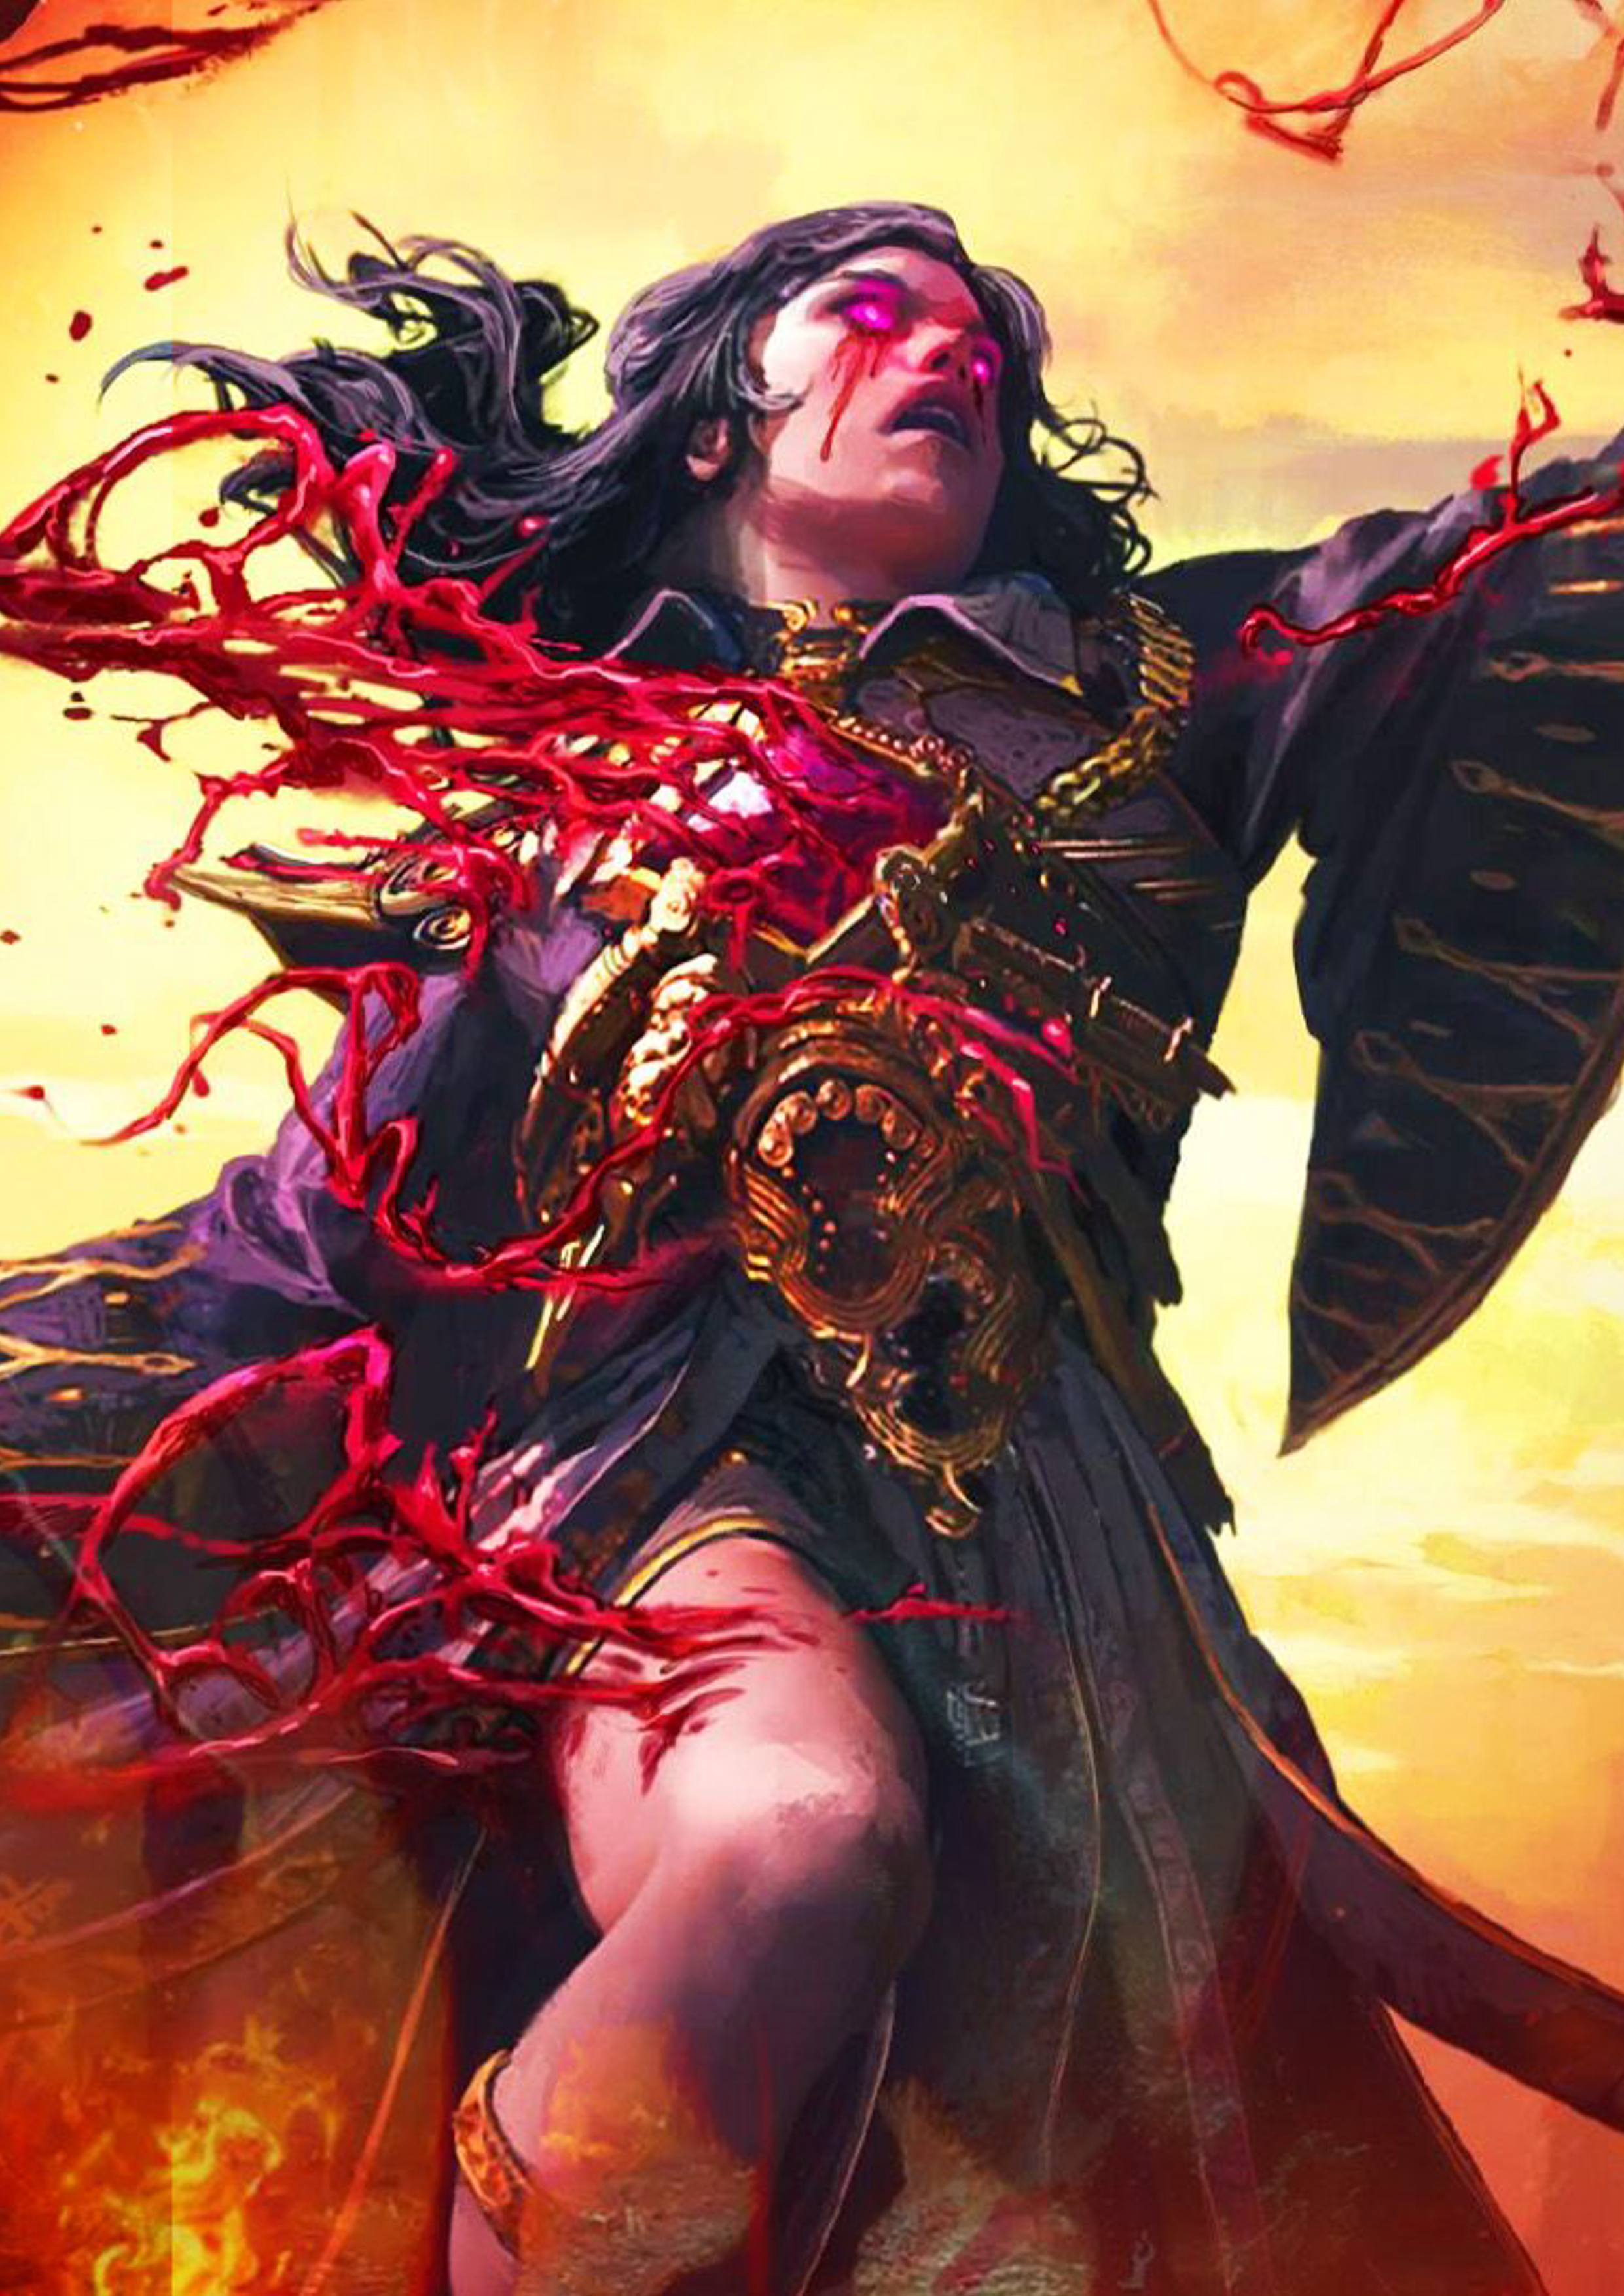
\includegraphics[width=\paperwidth,height=\paperheight]{resources/Blood_mage_bg.pdf}};

\clearpage


% \tableofcontents
\begin{figure}
\begin{DndSidebar}[color=DmgLilac]{Core Blood Mage Traits}
\begin{DndTable}[color=DmgSlateGrey]{XX}
 Trait & Description \\
 Primary Ability  & Constitution \\
 Hit Point Die  & D8 per Blood Mage level \\
 Saving Throw Proficiencies  & Constitution and Charisma \\
 Skill Proficiencies  & \textit{Choose 2}: Arcana, Deception, History, Intimidation, Investigation, Persuasion, Survival \\
 Weapon Proficiencies & Simple Weapons \\
 Armour Training & Light armor \\
 Starting Equipment & \textit{Choose A or B}: (A) 2 Daggers, Leather Armour, 30 GP; or (B) 100 GP
\end{DndTable}  
\end{DndSidebar}
\end{figure}

\DndDropCapLine{B}{lood mage learned to conjure innate magic of living flesh in} order to crush enemies and heal allies. Their magic appears brutal and primitive at first, but shows surprising sophistication when used by a skilled wielder. 
Geared toward battle, each spell is a balancing act between death and outstanding power sourced by sacrificing pieces of the very vessel caster inhabits. 



\subsection{Becoming a Blood Mage ...}
\subsubsection{As a Level 1 Character}
  \begin{itemize}
    \item Gain all the traits in the Core Blood Mage Traits table.
    \item Gain the Blood Mage's level 1 features, which are listed in the Blood Mage's Features table.
  \end{itemize}
\subsubsection{As a Multiclass Character}
  \begin{itemize}
    \item Gain the following traits from the Core Blood Mage Traits table: Hit Point Die and training with Light armor
    \item Gain the Blood Mage's level 1 features, which are listed in the Blood Mage's Features table. See the multiclassing rules in chapter 2 of Player's Handbook to determine your available spell slots.
  \end{itemize}

\begin{figure}[t]
  \includegraphics[scale=0.7]{resources/Blood_mage_right_transparent.png}
\end{figure}

\tikz[remember picture,overlay, blend mode=multiply] \node[anchor=north east, inner sep=0pt] at (current page.north east) {\includegraphics[scale=0.8]{resources/Blood_mage_right.png}};

\subsection{Blood Mage Class Features}

\subsubsection{Level 1: Carnal Invocations}

Hidden properties of living flesh allow Blood Mage to invoke their gruesome powers. You pick one invocation of your choice.
Invocations are described in the "Carnal Invocation Options" section later in this class's description.

\paragraph{Replacing and Gaining Invocations} Whenever you gain a Blood Mage level, you can replace one of your invocations with another one. 

When you gain certain Blood Mage levels, you gain more invocations of your choice, as shown in the Invocations column of the Blood Mage Features table.

You can't pick the same invocation more than once unless its description says otherwise.

\subsubsection{Level 1: Magic Of Flesh}

You gain spell-casting. See chapter 7 for the rules on Spellcasting. The information below details how you use those rules with Blood Mage spells, which appear in the Blood Mage spell list later in the class's description.

\paragraph{Cantrips} You know two cantrips of your choice. Whenever you gain a Blood Mage level, you can replace one of your cantrips from this feature with another cantrip of your choice.

When you reach Blood Mage level 4, you learn another cantrip of your choice, as shown in the Cantrips column of the Blood Mage features table.

\paragraph{Spell Slots} The Blood Mage features table shows how many spell slots you have to cast your Blood Mage spells of levels 1-2. The table also shows the level of those slots, all of which are the same level. 

\paragraph{Prepared Spells of Level 1+} You prepare the list of level 1+ spells that are available for you to cast with this feature. To start, choose two level 1 Blood Mage spells. 


The number of spells on your list increases as you gain Blood Mage levels, as shown in the Prepared Spells column of the Blood Mage Features table. Whenever that number increases, choose additional Blood Mage spells until the number of spells on your list matches the number in the table. The chosen spells must be of a level no higher than what's shown in the table's Slot Level column for your level. When you reach level 6, for example, you learn a new Blood Mage spell, which can be of levels 1-3.


If another Blood Mage feature gives you spells that you always have prepared, those spells don't count against the number of spells you can prepare with this feature, but those spells otherwise count as Blood Mage spells for you.


\tikz[remember picture,overlay, blend mode=multiply] \node[anchor=north, inner sep=-2pt] at (current page.north) {\includegraphics[scale=1.35]{resources/Blood_mage_top.png}};

\begin{table*}[ht]
  \includegraphics[scale=1.0]{resources/Blood_mage_top_tranparent.png}

  \caption{\DndFontTableTitle{Blood Mage Features}}\label{tab:bm_features}

  \begin{tabularx}{\linewidth}{p{0.7cm}p{2cm}Xp{2cm}p{1.5cm}p{1.5cm}p{1cm}p{1cm}}
    \textbf{Level}                  & \textbf{Proficiency bonus} & \textbf{Class Features} & \textbf{Carnal Invocations} & \textbf{Cantrips} & \textbf{Prepared Spells} & \textbf{Spell Slots} & \textbf{Slot Level}\\
 1                & +2 & Carnal Invocations, Magic of Flesh & 1 & 2 & 2 & 1 & 1 \\
 2                & +2 & Hemorrhage & 3 & 2 & 3 & 2 & 1 \\
 3                & +2 & Blood channelling, Spells of a mortal vessel & 3 & 2 & 4 & 2 & 2 \\
 4                & +2 & -- & 3 & 3 & 5 & 2 & 2 \\
  \end{tabularx}
\end{table*}

\paragraph{Changing Your Prepared Spells} Whenever you gain a Blood Mage level, you can replace one spell on your list with another Blood Mage spell of an eligible level.

\paragraph{Spellcasting Ability} Constitution is the spell-casting ability for your Blood Mage spells.

\paragraph{Spellcasting Focus} You can use your body as a Spellcasting Focus for your Blood Mage spells if you are not at full health.

\subsubsection{Level 2: Spell Carving}

Blood mage can carve spells on their own body using their skin as a makeshift Spell Scroll. Carving ritual could be done only during the Long Rest at a cost of healing. 

\paragraph{Prerequisites} You can perform the ritual by yourself or request assistance. You can scribe any spells that you know and have prepared or, if assisted, any spell that the assisting character knows.
Prerequisites about Scribing Spell Scroll from Player Handbook apply to either of you who knows the spell.

\paragraph{Time and Cost} One Long Rest counts as one day of work(8h) the cost is the same as for usual Spell Scroll. 

\paragraph{Casting carved spell} 
The carved spell is used as if it's on a Spell Scroll that you can't part with. 
Unlike the Spell Scroll you can cast it even if you don't know the spell and it still consumes a spell slot.
If somebody else casts it, by reading it off you for example, the spell slot is not consumed, but the spell must be in their spell list.  

\subsubsection{Level 3: Spells Of a Mortal Vessel}

Some spells are naturally compatible with your source of magical powers, that ensures you always have certain spells ready; Upon reaching 3rd Blood Mage level, you thereafter always have this listed spells prepared.

\begin{itemize}
  \item False Life
  \item Hellish Rebuke
  \item Arcane Vigor
  \item Warding Bond
\end{itemize}

\subsubsection{Level 3: Blood Channelling}

You can cast a spell without expending a spell slot; however, per spell slot level, you must either receive a Fatigue Level or take 1d12 necrotic damage that can't be prevented or reduced. 
If this action damage reduces you to 0 hit points or you lose consciousness, the spell fails. That includes carved spells from Spell Carving Trait.

While you have Fatigue condition you experience the following effects.

\paragraph{Fatigue Levels} This condition is cumulative. Each time you receive it, you gain 1 Fatigue Level. 
\paragraph{Weakness} When you receive non-necrotic damage, you receive additional one necrotic damage per Fatigue Level.
\paragraph{Decay} Your maximum health is reduced by 5 times your Fatigue Level.
\paragraph{Removing Fatigue} Finishing Long Rest removes all your Fatigue Levels. Finishing Short Rest removes half your Fatigue levels rounded up. Succeeding Death Saving Throw removes one Fatigue Level.

\begin{figure}[t]
  \includegraphics[scale=0.2]{resources/Blood_mage_corner_img_transparent.png}
\end{figure}
\tikz[remember picture,overlay, blend mode=multiply] \node[anchor=north west, inner sep=0pt] at (current page.north west) {\includegraphics[scale=0.25]{resources/Blood_mage_corner_img.png}};

\subsection{Carnal Invocation Options}

\subsubsection{Blood Is the Ultimate Sacrifice}

When casting a spell, you can choose to forego its material component. Take 1d12 necrotic damage per 50 GP of material. This damage can’t be reduced or prevented. 
If this damage reduces you to 0 hit points, the spell fails, but the spell slot is not expended.

\subsubsection{Wounds Mean Nothing To Me}

As a Magical Action, if not wearing any armor, Blood Mage can have their AC equal to 10 plus their dexterity modifier plus one per 5 missing Hit Points. 

The invocation ends early if Blood Mage dons armor.

Duration: 10 minutes.

\subsubsection{My Flesh Is Your Flesh}

Upon receiving damage from an attack, you can choose to turn your pain inside out, healing creatures around you. 

As a Reaction, for every 3 points of damage received, you can restore 1d4 Hit Points to any number of creatures other than you in a 5-foot radius.

\subsubsection{Summon Wound Shaped Weapon}

Upon receiving damage from a non-magical melee attack, Blood Mage can use Reaction to conjure a magical weapon that follows the shape of the wound. 

It looks and behaves like a copy of the melee weapon used in the attack and deals necrotic damage equal to the physical damage received by the Blood Mage. It becomes magical, gains Finesse property, and Blood Mage has proficiency with it. 

The weapon lasts 10 minutes or until it is out of Blood Mage's hands for more than 15 seconds. Blood Mage can dismiss the weapon at any time.

\subsubsection{Shared Suffering is Double Suffering}

As a Bonus Action, Blood Mage can touch a willing creature that is not full health. They suffer 1d8 necrotic damage per 5 missing Hit Points, and the Blood Mage regains that many Hit Points. 

\subsubsection{Pain Tribute Symbol}

As a Magical Action, Blood Mage can hurt themselves to reinforce a piece of equipment by drawing powers within his body. Blood Mage receives 1d8 damage and draws a symbol on a chosen surface, increasing its durability.

If it is a shield or a piece of armor, the wearer receives +1 AC. 

Only one Pain Tribute Symbol can be active at any given time. If the symbol is removed, for example if character falls into the water, effect ends.

%  My Injury Is My Strength
\subsubsection{Strength In Injury}

As a Magical Action, Blood Mage can sacrifice his flesh to receive temporary boost in strength. 
Choose a willing creature and number of d6 dice up to your Blood Mage Level and roll them all at once, you lose half that much Hit Points and chosen creature receives that much as a Temporary Hit Points. 
If you don't have that many Hit Points invocation is successful, but you die.

Range: Touch.

\subsubsection{Let the Blade Drink}

As a Bonus Action, you soak a blade of a non-magical weapon in your blood, taking 1d4 + 1 necrotic damage.
Until the effect ends, that weapon becomes a magic weapon with a +1 bonus to attack rolls and +2 to damage rolls. 
The spell ends early if you cast it again.

Duration: 1 hour?

\subsection{Blood Mage Spell List}

\begin{DndTable}[header=Cantriips(Level 0 Blood Mage Spells)]{XXX}
 Spell  & School & Special \\
 Thorn Whip & Transmutation & -- \\
 Blade Ward & Abjuration & C \\
 Eldritch Blast & Evocation & -- \\
 Chill Touch & Necromancy & -- \\
 Acid Splash & Evocation & -- \\
 Mind Sliver & Enchantment & -- \\
 Mage Hand & Conjugation & -- \\
 Poison Spray &  Necromancy & -- \\
 Prestidigitation & Transmutation & -- \\
\end{DndTable}

\begin{DndTable}[header=Level 1 Blood Mage Spells]{XXX}
 Spell  & School & Special \\
 Chromatic Orb & Evocation & -- \\
 False Life & Necromancy & -- \\
 Hellish Rebuke & Evocation & --\\
 Ice Knife & Conjuration & -- \\
 Identify & Divination & R \\
 Inflict Wounds & Necromancy & -- \\
 Shield & Abjuration & -- \\
 Unseen Servant & Conjuration & R \\
 Compelled Duel & Enchantment & C \\
 Tasha's Hideous Laughter & Enchantment & C \\
\end{DndTable}

\begin{DndTable}[header=Level 2 Blood Mage Spells]{XXX}
 Spell  & School & Special \\
 Arcane Vigor & Abjuration & -- \\
 Barkskin & Transmutation & -- \\
 Knock & Transmutation & -- \\
 Magic Weapon & Transmutation & -- \\
 Warding Bond & Abjuration & -- \\
 Alter Self & Transmutation & C \\
 Enhance Ability & Transmutation & C \\
 Mind Spike & Divination & C \\
 Spike Growth & Transmutation & C \\
 Shatter & Evocation & -- \\
 Heat Metal & Transmutation & C \\
 Misty Step & Conjugation & -- \\
\end{DndTable}

\maketitle

\end{document}